In the most straightforward form of Lazy Shadowing, each main is associated with one shadow. This is ignorant of the variance in the underlying hardware reliability and above application criticality. In fact, the computational model of Lazy Shadowing does not restrict how shadows should be associated with mains. In this chapter, we will explore smart shadowing techniques to make Lazy Shadowing adaptive, in the sense of dynamically harnessing all available resources to achieve the highest level of QoS. 

Previous studies have shown that failure rates both vary across systems and vary across nodes within the same system~\cite{schroeder2007,di2014lessons}. According to \cite{di2014lessons}, 19\% of the nodes account for 92\% of the machine check errors on Blue Waters. The reason for the non-uniform distribution of failure is complicated and may attribute to the manufacture process, heterogeneous architecture, environment factors (e.g. temperature, voltage supply), and/or workloads. At the same time, within a system processes may have different criticality. One possible reason is that the execution model assigns different roles to different processes. For example, the master process in the master-slave execution model is a single point of failure, making the failure of the master process more severe than failure of a slave process. Another possibility is when the user have the option to specify the QoS. For example, in Cloud Computing, users may choose differernt level of QoS in terms of Service Level Agreement with different amount of payment. 

There are two aspects of Lazy Shadowing that we can customize in order to adapt to the hardware, workload, and QoS requirement. Firstly, in a system where CPU cores have different propensity to failures, mapping from processes to physical cores will largely impact the successful execution of each process. For Lazy Shadowing, it is a non-trival question to decide the mapping for both main and shadow processes. Secondly, Lazy Shadowing allows different tasks to use different number of shadows. Within the resource limitation, more shadows would be allocated for more critical mains or mains that are more likely to fail. 

To explore smart shadowing, firstly I will study the failure distribution on real large-scale production systems. Using failure logs from the Computer Failure Data Repository~\cite{cfdr}, I will apply machine learing techniques to classify nodes based on their reliability and learn the distribution of each category. Then an optimization problem will be formulated to derive the optimal mapping and allocation (Figure~\ref{fig:opt_problem}). The inputs to the problem are system parameters and application parameters, the constraints are deadlines and limitation on resources, and the output are the process mapping and shadow allocation. Lastly, I will evaluate the results with trace based simulation.

\begin{figure}[!t]
  \begin{center}
      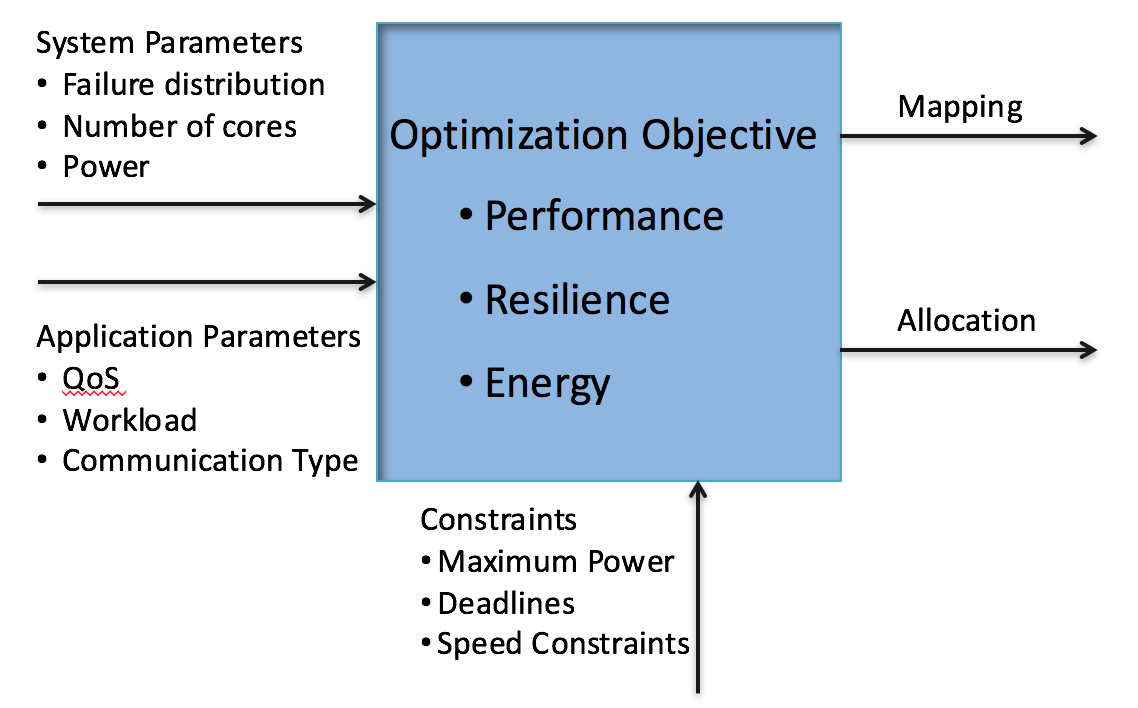
\includegraphics[width=0.7\columnwidth]{figures/opt_problem.png}
  \end{center}
  \caption{Optimization problem framework.}
  \label{fig:opt_problem}
\end{figure}